\section{DFR on $\mathcal{A}_{t,\ell}(\mathcal{S})$}

Recall that Vasseur identified three problematic sets of $(u,v)$-near codewords and proposed a study on the effect of proximity of error vectors to these sets by defining the set: $$\mathcal{A}_{t,\ell}(\mathcal{S}) := \{v \in \FF_2^{2r} : |v \star c| = \ell \text{ for some } c \in \mathcal{S} \}$$.

While $\ell$ measures the number of common intersections of an error vector with an element of $\mathcal{S}$, we can define another quantity that measures the distance of an error vector from $\mathcal{S}$:

\[
\delta(e) = |c| + t - 2\ell
\]

where $c\in \mathcal{S}$ is the vector with $|e \star c| = \ell$.

For $\ell$ high ( equivalently, $\delta$ low), decoding failures are extremely prevalent ( see Figure \ref{fig:DFR_CN2N}).

\begin{figure}[h]
    \centering
    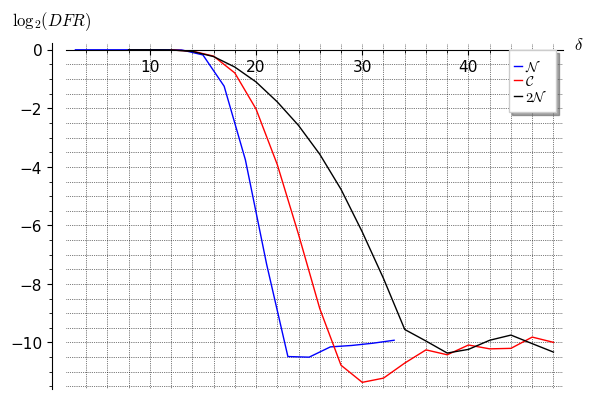
\includegraphics[scale=.75]{2_bike/DFR_20bit_CN2N_new.png}
    \caption{20-bit security DFR versus $\delta$ for near-codeword sets  $\mathcal{C},\mathcal{N}, 2\mathcal{N}$ for $r = 523$}
    \label{fig:DFR_CN2N}
\end{figure}

We study the relationship between $\mathcal{A}_{t,\ell}(\mathcal{S})$ for some $\ell$, $\mathcal{S} \in \{ \mathcal{C}, \mathcal{N}, 2\mathcal{N} \}$ and decoding failures. Our data shows that it is highly unlikely for a decoding failure vector to have a high intersection with an element in $\mathcal{S}$. For a vector $v$, we define the maximum overlap of $v$ for a fixed $\mathcal{S}$ by computing the largest $\ell$ such that $v \in \mathcal{A}_{t,\ell}(\mathcal{S})$. Using the experimental data from $r=587, N=10^9$ we recorded 557 total decoding failures and stored the 557 random error vectors that led to decoding failure. The relationship between these decoding failure vectors and the sets $\mathcal{S} $ is shown below:


\begin{figure}[htbp]
  \begin{center}
    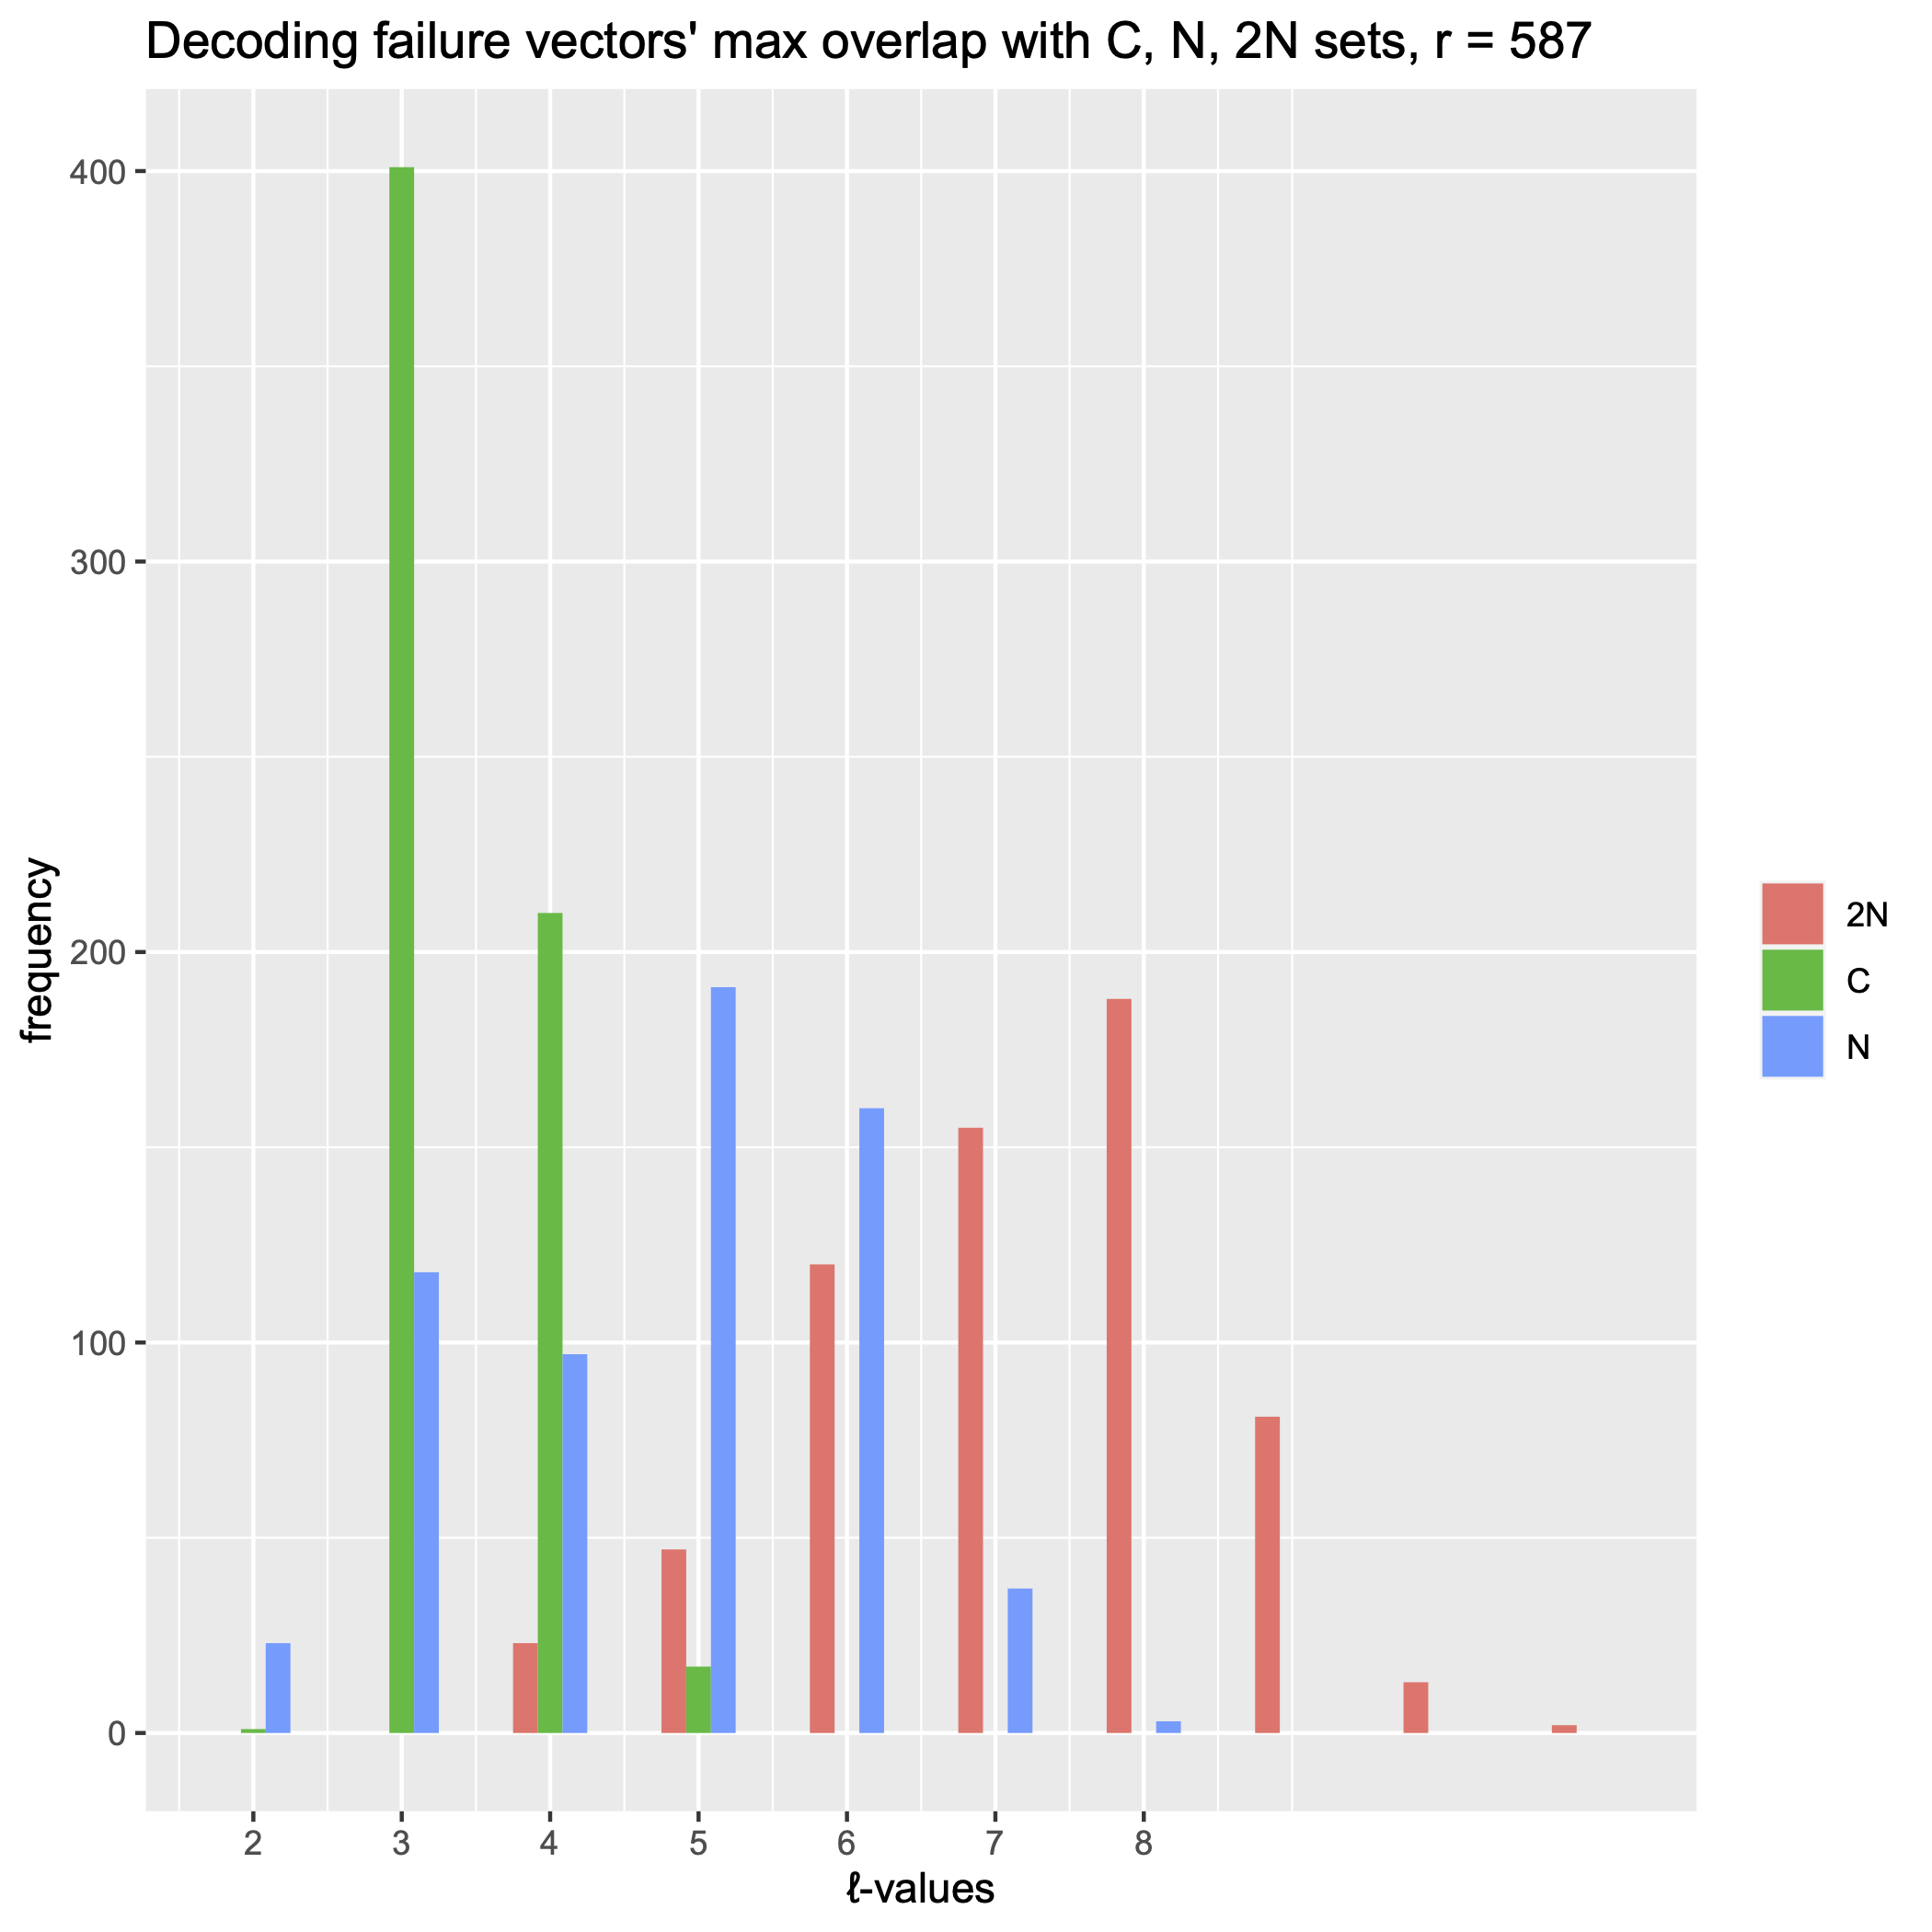
\includegraphics[width=0.49\textwidth]{2_bike/Rplot-587-df.png}
    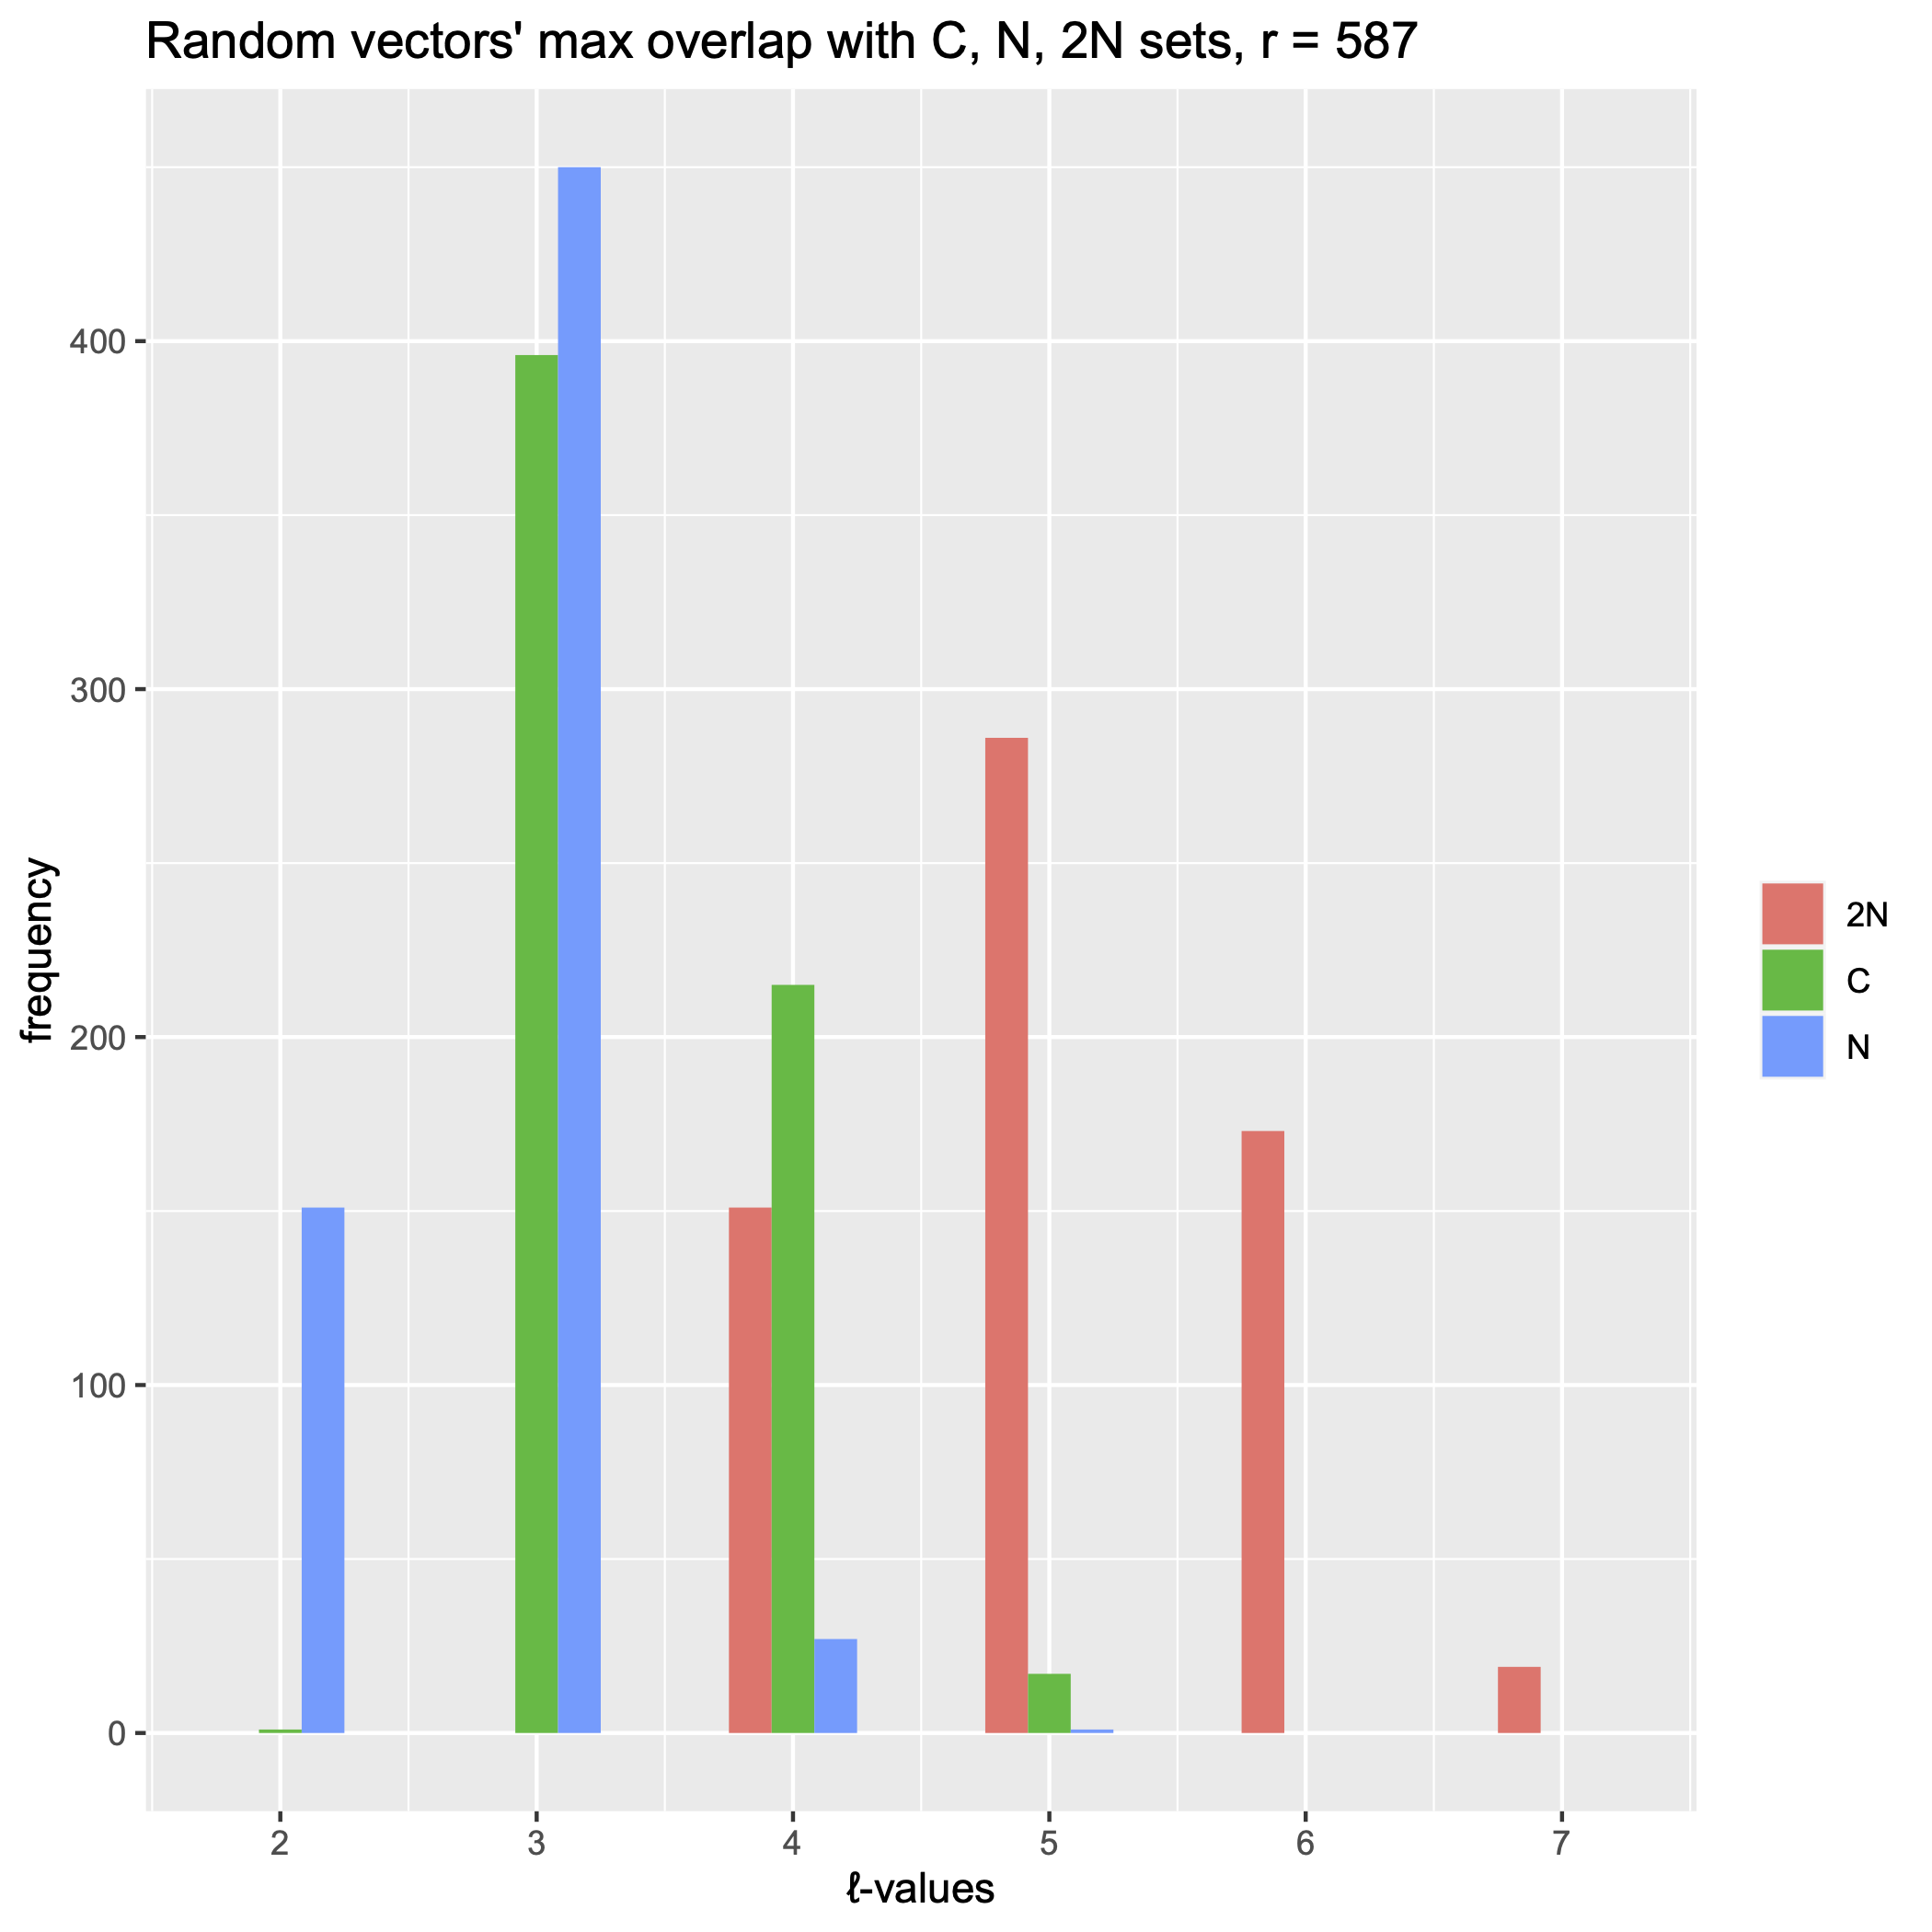
\includegraphics[width=0.49\textwidth]{2_bike/Rplot-587-random.png}
  \end{center}
  \caption{Distribution of maximum overlaps of decoding failure vectors (left) or random vectors (right) with the sets $\mathcal{C}$, $\mathcal{N}$, and $2\mathcal{N}$ for $r = 587$, using a weak key threshold of $T = 3$ to generate keys.}
  \label{fig:AtlS}
\end{figure}

The cases where $\ell > 10$ are rare. It is expected that these problematic sets contribute to the decoding failures occuring in error floor region and our data suggests that some proportion of decoding failures can be explained by their proximity to $\mathcal{N}$ or $2\mathcal{N}$. However, it is also the case that a significant of the errors causing decoding failures do not have more overlap with $\mathcal{S}$ than typical random vectors. Further analysis is needed to determine what proportion of decoding failures are explained by this proximity.